% ============================================================
% 11-bezier-quadratic-makie-explained.tex
% Compile with:  pdflatex -shell-escape 11-bezier-quadratic-makie-explained.tex
% The PNG file must be in the same folder as this .tex file.
% Run twice for table of contents.
% ============================================================

\documentclass[12pt, a4paper]{article}

\usepackage[T1]{fontenc}
\usepackage[utf8]{inputenc}
\usepackage{lmodern}
\usepackage[top=2.5cm, bottom=2.5cm, left=2.8cm, right=2.8cm]{geometry}
\usepackage{graphicx}
\usepackage{float}
\usepackage[dvipsnames]{xcolor}

\definecolor{codebg}{RGB}{248,248,248}
\definecolor{rulecolor}{RGB}{180,180,180}
\definecolor{examplebg}{RGB}{240,248,255}
\definecolor{examplerule}{RGB}{100,149,237}
\definecolor{notebg}{RGB}{255,250,230}
\definecolor{noterule}{RGB}{210,180,50}
\definecolor{diffbg}{RGB}{240,255,240}
\definecolor{diffrule}{RGB}{80,160,80}

\usepackage{minted}
\setminted[julia]{
  bgcolor=codebg, frame=leftline, framerule=1.5pt,
  rulecolor=rulecolor, linenos=false, fontsize=\small,
  breaklines=true, tabsize=4, style=friendly,
}

\usepackage{amsmath}
\usepackage{amssymb}
\usepackage{tikz}
\usetikzlibrary{shapes.geometric, arrows.meta, positioning}
\usepackage{mdframed}

\newmdenv[backgroundcolor=examplebg, linecolor=examplerule,
  linewidth=1.5pt, leftline=true, rightline=false,
  topline=false, bottomline=false,
  innerleftmargin=10pt, innerrightmargin=8pt,
  innertopmargin=6pt, innerbottommargin=6pt,
  skipabove=6pt, skipbelow=4pt]{examplebox}

\newmdenv[backgroundcolor=notebg, linecolor=noterule,
  linewidth=1.5pt, leftline=true, rightline=false,
  topline=false, bottomline=false,
  innerleftmargin=10pt, innerrightmargin=8pt,
  innertopmargin=6pt, innerbottommargin=6pt,
  skipabove=6pt, skipbelow=4pt]{notebox}

\newmdenv[backgroundcolor=diffbg, linecolor=diffrule,
  linewidth=1.5pt, leftline=true, rightline=false,
  topline=false, bottomline=false,
  innerleftmargin=10pt, innerrightmargin=8pt,
  innertopmargin=6pt, innerbottommargin=6pt,
  skipabove=6pt, skipbelow=4pt]{diffbox}

\usepackage[colorlinks=true, linkcolor=black, urlcolor=MidnightBlue]{hyperref}
\usepackage{booktabs}
\usepackage{needspace}
\usepackage{parskip}
\usepackage{titlesec}
\usepackage{fancyhdr}
\usepackage{datetime2}

\titleformat{\section}
  {\large\bfseries\color{MidnightBlue}}{\thesection.}{0.6em}{}
  [\vspace{-4pt}\rule{\linewidth}{0.4pt}]
\titleformat{\subsection}
  {\normalsize\bfseries\color{BrickRed}}{\thesubsection.}{0.5em}{}
\titleformat{\subsubsection}
  {\normalsize\bfseries}{\thesubsubsection.}{0.5em}{}

\pagestyle{fancy}
\fancyhf{}
\rhead{\textcolor{gray}{\small 11-bezier-quadratic-makie-explained}}
\lhead{\textcolor{gray}{\small B\'ezier Quadratic --- CairoMakie}}
\cfoot{\thepage}
\renewcommand{\headrulewidth}{0.3pt}

\newcommand{\cd}[1]{\texttt{#1}}

\title{%
  \vspace{1cm}
  {\LARGE\bfseries B\'ezier Curve: Quadratic (2-D)}\\[0.4em]
  {\large CairoMakie Visualisation}\\[0.4em]
  {\large Code and Plot Explanation for Julia Beginners}\\[0.4em]
  {\normalsize\texttt{11-bezier-quadratic-makie.jl}}
}
\author{E.R.\ Nurwijayadi}
\date{\DTMtoday}

\begin{document}

\maketitle
\thispagestyle{empty}

\begin{center}
\textit{Directed and curated by E.R.\ Nurwijayadi.
Code and explanations AI-generated.}
\end{center}

\begin{center}
\begin{minipage}{0.85\textwidth}
\small
This document explains \cd{11-bezier-quadratic-makie.jl}.
It is the CairoMakie counterpart to
\cd{11-bezier-quadratic-plots.jl}.
The curve, control points, and all computed values are
identical --- only the plotting library and its API differ.
This document is fully self-contained but deliberately
highlights the differences from Plots.jl
so you can read the two side by side.
\end{minipage}
\end{center}

\vspace{1em}\hrule\vspace{1.5em}
\tableofcontents
\newpage


% =============================================================
\needspace{8\baselineskip}
\section{The Plot}
% =============================================================

\begin{figure}[H]
  \centering
  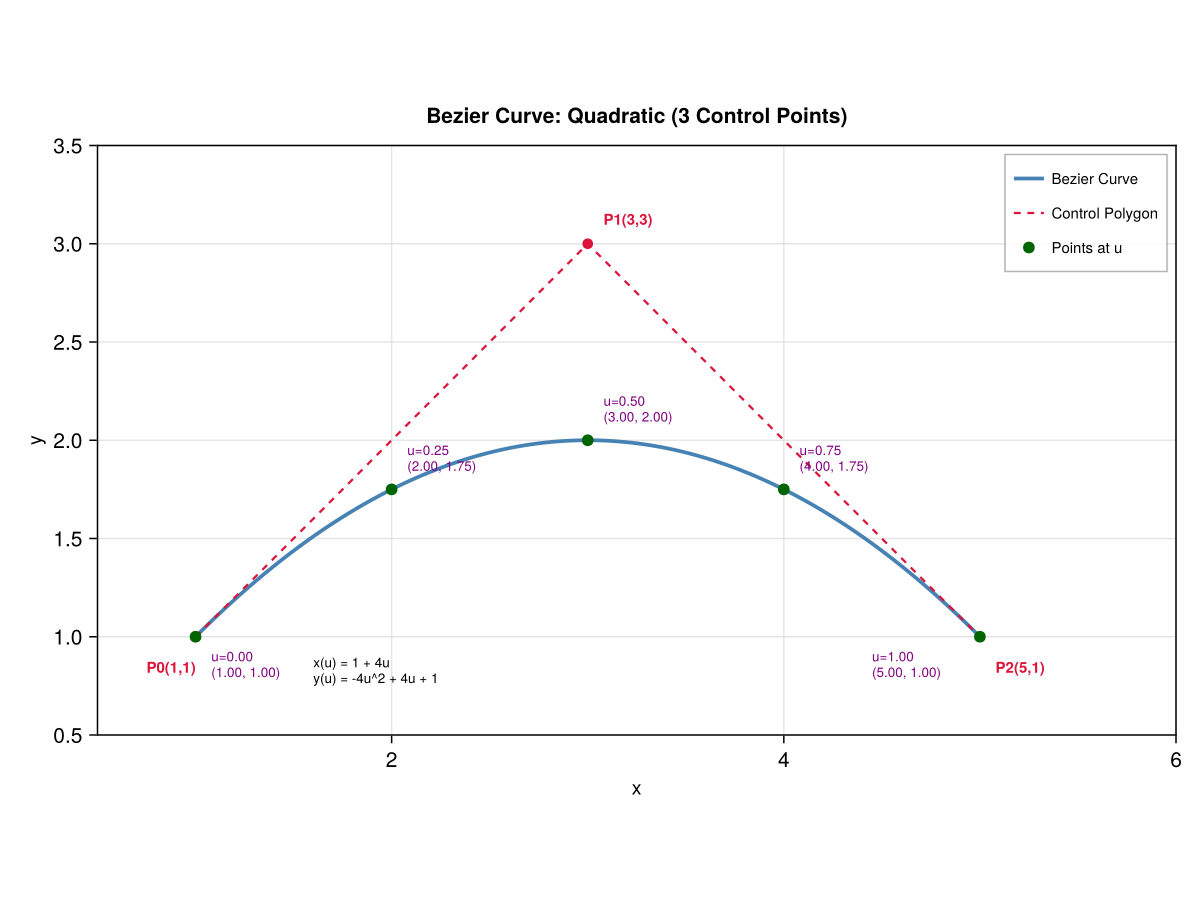
\includegraphics[width=0.95\linewidth]{11-bezier-quadratic-makie.png}
  \caption{Quadratic B\'ezier curve with 3 control points,
           plotted with CairoMakie.}
  \label{fig:bezier-quadratic-makie}
\end{figure}


% =============================================================
\needspace{8\baselineskip}
\section{Reading the Plot}
% =============================================================

The content is identical to the Plots.jl version:
the same blue curve, red dashed control polygon,
green highlighted dots, purple annotations, and
equation text.
The geometric meaning is unchanged.

\needspace{5\baselineskip}
\subsection{Visual differences from the Plots.jl version}

Looking at the two plots side by side, several visual
differences are immediately visible:

\begin{center}
\begin{tabular}{lll}
\toprule
Element & Plots.jl & CairoMakie \\
\midrule
Frame & Four-sided box & Open axes (no right/top border) \\
Title font & Normal weight & \textbf{Bold} \\
Background & White with grid & White with lighter grid lines \\
Control polygon markers & Medium circles & Slightly larger circles \\
Resolution & 800$\times$600 px & 800$\times$600 $\times$ 1.5 = 1200$\times$900 px \\
Legend & Inside plot area & Separate legend box, top-right \\
\bottomrule
\end{tabular}
\end{center}

These differences come entirely from the two libraries'
default styling and rendering engines, not from any
difference in the underlying curve data.

\begin{notebox}
\textbf{CairoMakie vs Plots.jl rendering.}
Plots.jl uses the GR backend by default, which renders
to screen at 1:1 pixel ratio.
CairoMakie uses Cairo, a vector graphics library,
and the \cd{px\_per\_unit = 1.5} argument in \cd{save()}
produces a higher-resolution PNG: $800 \times 1.5 = 1200$
pixels wide instead of 800.
This is why the CairoMakie output looks sharper.
\end{notebox}


% =============================================================
\needspace{8\baselineskip}
\section{What is CairoMakie?}
% =============================================================

\textit{Makie is Julia's other major plotting framework.
Understanding how it differs from Plots.jl explains why
the code looks so different even though it draws the same thing.}

\textbf{Makie.jl} is a \emph{native Julia} plotting framework
built from the ground up for performance and flexibility.
It does not wrap another library --- it renders directly
using its own scene graph.
There are three backends:

\begin{center}
\begin{tabular}{lp{8.5cm}}
\toprule
Backend & Use case \\
\midrule
\cd{CairoMakie} &
  Static output to PNG, SVG, PDF.
  Uses the Cairo library. Good for publication-quality figures. \\
\cd{GLMakie} &
  Interactive plots in a GPU-accelerated window.
  Good for real-time updates and 3-D rotation. \\
\cd{WGLMakie} &
  Interactive plots in a web browser via WebGL.
  Good for Jupyter notebooks and web deployment. \\
\bottomrule
\end{tabular}
\end{center}

This script uses \cd{CairoMakie} because it saves to PNG
without needing a display server.

\textbf{The key architectural difference from Plots.jl:}
In Plots.jl, \cd{plot()} creates and returns a plot object
that is both the figure and the axes combined.
In Makie, these are always separate:
\cd{Figure} is the canvas, \cd{Axis} is a coordinate system
placed inside the figure.
This separation gives much finer control over layout.

Install once with:
\begin{minted}{julia}
import Pkg; Pkg.add("CairoMakie")
\end{minted}


% =============================================================
\needspace{8\baselineskip}
\section{Type Map}
% =============================================================

\tikzset{
  structbox/.style={rectangle, rounded corners=4pt,
    draw=MidnightBlue, line width=1.5pt, fill=examplebg,
    text width=3.2cm, align=center, font=\small\bfseries, inner sep=8pt},
  funcbox/.style={rectangle, rounded corners=2pt,
    draw=gray!60, line width=1pt, fill=white,
    text width=3.2cm, align=center, font=\small, inner sep=7pt},
  entrybox/.style={rectangle, rounded corners=4pt,
    draw=BrickRed, line width=1.5pt, fill=notebg,
    text width=2.4cm, align=center, font=\small\bfseries, inner sep=8pt},
  myarrow/.style={-Stealth, thick, draw=gray!70},
  bluearrow/.style={-Stealth, thick, draw=MidnightBlue},
  redarrow/.style={-Stealth, thick, draw=BrickRed!80},
  arrowlabel/.style={font=\footnotesize\itshape, fill=white, inner sep=2pt}
}

\begin{center}
\begin{tikzpicture}[node distance=1.4cm and 2.6cm]

  \node[structbox] (bz) {%
    \texttt{BezierQuadratic}\\[3pt]
    \footnotesize\normalfont
    \texttt{p0, p1, p2}\\
    \texttt{::Vector\{Float64\}}
  };

  \node[funcbox, below left=1.5cm and 0.4cm of bz] (math) {%
    \textbf{Math functions}\\[2pt]
    \footnotesize\normalfont
    \texttt{point(bz, u)}\\
    \texttt{curve(bz, n)}\\
    \texttt{highlight\_points}
  };

  \node[funcbox, below right=1.5cm and 0.4cm of bz] (draw) {%
    \texttt{draw\_and\_save}\\[2pt]
    \footnotesize\normalfont
    \textit{Figure + Axis layout}\\
    \textit{layers: lines!, scatter!}\\
    \textit{text!, axislegend, save}
  };

  \node[entrybox, right=2.2cm of bz] (main) {%
    \texttt{main()}\\[2pt]
    \footnotesize\normalfont\normalcolor
    \textit{entry point}
  };

  \draw[bluearrow] (bz)   -- node[arrowlabel,above left]{passed to} (math);
  \draw[bluearrow] (bz)   -- node[arrowlabel,above right]{passed to} (draw);
  \draw[myarrow]   (draw) -- node[arrowlabel,below]{calls} (math);
  \draw[redarrow]  (main) -- node[arrowlabel,above]{creates} (bz);
  \draw[redarrow]  (main) |- node[arrowlabel,right,pos=0.8]{calls} (draw);

\end{tikzpicture}
\end{center}

The structure is identical to the Plots.jl version.
Only the internals of \cd{draw\_and\_save} changed.


% =============================================================
\needspace{8\baselineskip}
\section{Data, Constants, and Math Functions}
% =============================================================

\cd{CONTROL\_POINTS}, \cd{U\_HIGHLIGHT}, \cd{U\_OFFSETS},
the colour constants, \cd{BezierQuadratic} (struct and
constructor), \cd{curve}, and \cd{highlight\_points}
are \textbf{identical} to the Plots.jl version.
Please refer to \cd{11-bezier-quadratic-plots-explained}
for full explanations of those components.

One small difference: \cd{point()} no longer calls a
separate \cd{basis()} function.
The Bernstein weights are computed inline:

\begin{minted}{julia}
function point(bz::BezierQuadratic, u::Float64)
    b0 = (1 - u)^2
    b1 = 2 * u * (1 - u)
    b2 = u^2
    b0 .* bz.p0 .+ b1 .* bz.p1 .+ b2 .* bz.p2
end
\end{minted}

This is functionally identical to the Plots.jl version
where \cd{b0, b1, b2 = basis(u)} was called first.
The computation and result are the same; the \cd{basis}
helper is simply not factored out as a separate function here.

\textbf{All data tables} (\cd{cpts}, \cd{cp}, \cd{hpts},
\cd{pt} values) are also identical to the Plots.jl version
since the math is unchanged.


% =============================================================
\needspace{8\baselineskip}
\section{\texttt{draw\_and\_save} --- The Makie Drawing API}
% =============================================================

\textit{This is where the two scripts diverge completely.
Makie separates figure, axes, and drawing into distinct steps.
Plots.jl collapsed all of these into a single \cd{plot()} call.}

\needspace{5\baselineskip}
\subsection{Step 1: Create the Figure}

\begin{minted}{julia}
fig = Figure(size = (800, 600), backgroundcolor = :white)
\end{minted}

\cd{Figure} is the top-level canvas.
It has a size and a background colour, but it does not yet
have any coordinate system or data.
Think of it as a blank sheet of paper.

\begin{diffbox}
\textbf{Plots.jl:} \cd{plt = plot(size=(800,600), background=:white, ...)}
--- one call creates figure, axes, and layout all at once.

\textbf{CairoMakie:} \cd{fig = Figure(...)} creates only the canvas.
The axes are created separately in the next step.
\end{diffbox}

\needspace{5\baselineskip}
\subsection{Step 2: Create the Axis}

\begin{minted}{julia}
ax = Axis(fig[1, 1],
    title           = "Bezier Curve: Quadratic (3 Control Points)",
    titlesize       = 14,
    titlegap        = 12,
    xlabel          = "x",
    ylabel          = "y",
    xlabelsize      = 13,
    ylabelsize      = 13,
    limits          = (0.5, 6.0, 0.5, 3.5),
    aspect          = DataAspect(),
    xgridcolor      = (:lightgray, 0.6),
    ygridcolor      = (:lightgray, 0.6),
    backgroundcolor = :white,
)
\end{minted}

\textbf{\cd{fig[1, 1]}:}
Makie uses a \textbf{grid layout} to place axes inside a figure.
\cd{fig[1, 1]} means row 1, column 1 of the figure grid.
A figure can hold multiple axes in different grid positions
(e.g.\ \cd{fig[1,1]}, \cd{fig[1,2]}, \cd{fig[2,1]} for a
$2 \times 2$ grid of subplots).
Here there is only one axis, placed at position $(1,1)$.

\textbf{\cd{limits = (xmin, xmax, ymin, ymax)}:}
Sets the visible range of the axes.
In Plots.jl this was two separate keyword arguments
\cd{xlims} and \cd{ylims}.
Makie combines them into one 4-tuple.

\textbf{\cd{aspect = DataAspect()}:}
Forces equal scaling of $x$ and $y$ axes, just like
\cd{aspect\_ratio = :equal} in Plots.jl.
\cd{DataAspect()} is a Makie type that means
``use the data coordinate ratio, not the pixel ratio.''

\textbf{\cd{xgridcolor = (:lightgray, 0.6)}:}
Makie accepts colours as \textbf{(name, alpha)} tuples.
\cd{(:lightgray, 0.6)} means light gray at 60\% opacity.
In Plots.jl the equivalent was separate \cd{gridcolor}
and \cd{gridalpha} arguments.

\begin{examplebox}
\textbf{The grid layout system:}

A single plot looks like this in memory:
\begin{minted}{julia}
fig = Figure(...)          # canvas (blank paper)
ax  = Axis(fig[1,1], ...)  # axes at grid position (1,1)
\end{minted}

A two-column subplot layout would be:
\begin{minted}{julia}
ax1 = Axis(fig[1,1], ...)  # left axes
ax2 = Axis(fig[1,2], ...)  # right axes
\end{minted}

This grid system is why Makie is preferred for complex
multi-panel figures.
\end{examplebox}

\needspace{5\baselineskip}
\subsection{Step 3: Draw the Curve --- \texttt{lines!}}

\begin{minted}{julia}
cpts = curve(bz)
lines!(ax, cpts[:,1], cpts[:,2],
    color     = COLOR_CURVE,
    linewidth = 2.5,
    label     = "Bezier Curve",
)
\end{minted}

In Makie, \cd{lines!} is the explicit function for drawing
a connected line through a series of points.
The first argument is the \textbf{axis} \cd{ax}, not the
figure or a plot object.

\begin{diffbox}
\textbf{Plots.jl:} \cd{plot!(plt, xs, ys, ...)}
--- \cd{plot!} is a generic function that draws a line
by default; the type of plot is inferred from options.

\textbf{CairoMakie:} \cd{lines!(ax, xs, ys, ...)}
--- the function name explicitly states what is drawn.
Makie has separate functions: \cd{lines!} for lines,
\cd{scatter!} for points, \cd{band!} for filled regions, etc.
There is no generic \cd{plot!} that guesses the type.
\end{diffbox}

The \cd{cpts} matrix is identical to the Plots.jl version:
$200 \times 2$, with \cd{cpts[:,1]} the $x$ column and
\cd{cpts[:,2]} the $y$ column.

\needspace{5\baselineskip}
\subsection{Step 4: Draw the Control Polygon --- Two Separate Calls}

\begin{minted}{julia}
cp = vcat(bz.p0', bz.p1', bz.p2')
lines!(ax, cp[:,1], cp[:,2],
    color     = COLOR_POLYGON,
    linestyle = :dash,
    linewidth = 1.5,
    label     = "Control Polygon",
)
scatter!(ax, cp[:,1], cp[:,2],
    color       = COLOR_POLYGON,
    markersize  = 10,
    strokewidth = 0,
)
\end{minted}

This is the most visible API difference from Plots.jl.

In Plots.jl, one \cd{plot!} call with \cd{marker = :circle}
drew both the dashed line \emph{and} the circles at the
control points.

In Makie, lines and scatter markers are always separate
drawing operations.
\cd{lines!} draws the dashed connecting line.
\cd{scatter!} draws the red circles at $P_0$, $P_1$, $P_2$.
The second \cd{scatter!} call has no \cd{label} argument ---
it should not appear in the legend separately because it is
part of the same ``Control Polygon'' visual element.

\begin{examplebox}
\textbf{Content of \cd{cp} (same as Plots.jl version):}

\[
  \cd{cp} =
  \begin{bmatrix}
    1.0 & 1.0 \\
    3.0 & 3.0 \\
    5.0 & 1.0
  \end{bmatrix}
\]

\cd{cp[:,1] = [1.0, 3.0, 5.0]} \quad --- $x$ coords of control points

\cd{cp[:,2] = [1.0, 3.0, 1.0]} \quad --- $y$ coords of control points
\end{examplebox}

\needspace{5\baselineskip}
\subsection{Step 5: Annotate Control Points --- \texttt{text!}}

\begin{minted}{julia}
offsets_ctrl = [(-0.25, -0.20), (0.08, 0.08), (0.08, -0.20)]
names_ctrl   = ["P0(1,1)", "P1(3,3)", "P2(5,1)"]
for (i, (name, (dx, dy))) in enumerate(zip(names_ctrl, offsets_ctrl))
    text!(ax, cp[i,1]+dx, cp[i,2]+dy,
        text     = name,
        color    = COLOR_CTRL,
        fontsize = 10,
        font     = :bold,
    )
end
\end{minted}

\textbf{\cd{text!} vs \cd{annotate!}:}
Makie uses \cd{text!} for placing labels.
The text string is passed as a keyword argument
\cd{text = name}, not as a positional argument.

\textbf{\cd{enumerate(zip(...))} with index \cd{i}:}
The loop uses \cd{enumerate} to get both the index \cd{i}
and the \cd{(name, (dx,dy))} tuple simultaneously.
This is because Makie's \cd{text!} needs the coordinates
in the form \cd{cp[i,1]} and \cd{cp[i,2]} --- indexing
by row number --- rather than \cd{eachrow(cp)} as in
the Plots.jl version.

\begin{diffbox}
\textbf{Plots.jl} used \cd{eachrow(cp)} to iterate over
row vectors, then accessed \cd{pt[1]} and \cd{pt[2]}.

\textbf{CairoMakie} uses \cd{enumerate(zip(...))} to get
the row index \cd{i}, then accesses \cd{cp[i,1]} and
\cd{cp[i,2]} directly.

Both achieve the same result.
The Makie version is slightly more explicit about the index.
\end{diffbox}

\needspace{5\baselineskip}
\subsection{Step 6: Highlighted Points and Labels}

\begin{minted}{julia}
hpts = highlight_points(bz, u_highlight)
scatter!(ax, hpts[:,1], hpts[:,2],
    color       = COLOR_POINT,
    markersize  = 11,
    strokewidth = 0,
    label       = "Points at u",
)
\end{minted}

\cd{strokewidth = 0} in Makie is the equivalent of
\cd{markerstrokewidth = 0} in Plots.jl ---
both remove the border ring around each marker.

\begin{examplebox}
\textbf{Content of \cd{hpts} (same as Plots.jl version):}

\[
  \cd{hpts} =
  \begin{bmatrix}
    1.00 & 1.00 \\
    2.00 & 1.75 \\
    3.00 & 2.00 \\
    4.00 & 1.75 \\
    5.00 & 1.00
  \end{bmatrix}
\]
\end{examplebox}

\begin{minted}{julia}
for u in u_highlight
    pt     = point(bz, u)
    x, y   = pt[1], pt[2]
    dx, dy = get(U_OFFSETS, u, (0.08, 0.08))
    text!(ax, x+dx, y+dy,
        text     = @sprintf("u=%.2f\n(%.2f, %.2f)", u, x, y),
        color    = COLOR_LABEL,
        fontsize = 9,
    )
end
\end{minted}

The loop logic is identical to Plots.jl.
The only difference is using \cd{text!(ax, x, y, text=...)}
instead of \cd{annotate!(plt, x, y, text(...))}.

\begin{examplebox}
\textbf{Value of \cd{pt} for each iteration (same as Plots.jl):}

\medskip
\begin{tabular}{ccccl}
\toprule
$u$ & \cd{pt[1]} & \cd{pt[2]} & Label text & Offset \\
\midrule
0.00 & 1.00 & 1.00 & \cd{u=0.00\textbackslash n(1.00, 1.00)} & $(+0.08,-0.22)$ \\
0.25 & 2.00 & 1.75 & \cd{u=0.25\textbackslash n(2.00, 1.75)} & $(+0.08,+0.08)$ \\
0.50 & 3.00 & 2.00 & \cd{u=0.50\textbackslash n(3.00, 2.00)} & $(+0.08,+0.08)$ \\
0.75 & 4.00 & 1.75 & \cd{u=0.75\textbackslash n(4.00, 1.75)} & $(+0.08,+0.08)$ \\
1.00 & 5.00 & 1.00 & \cd{u=1.00\textbackslash n(5.00, 1.00)} & $(-0.55,-0.22)$ \\
\bottomrule
\end{tabular}
\end{examplebox}

\needspace{5\baselineskip}
\subsection{Step 7: Equation Text}

\begin{minted}{julia}
text!(ax, 1.6, 0.75,
    text     = "x(u) = 1 + 4u\ny(u) = -4u^2 + 4u + 1",
    color    = :black,
    fontsize = 9,
)
\end{minted}

Identical in purpose to the Plots.jl version.
The position \cd{(1.6, 0.75)} is in data coordinates.
The \cd{\\n} produces a line break between the two equations.

\needspace{5\baselineskip}
\subsection{Step 8: The Legend --- \texttt{axislegend}}

\begin{minted}{julia}
axislegend(ax,
    position        = :rt,
    labelsize       = 10,
    framecolor      = (:black, 0.3),
    backgroundcolor = (:white, 0.8),
)
\end{minted}

In Plots.jl, the legend is configured as part of the
initial \cd{plot()} call with \cd{legend = :topright}.

In Makie, the legend is added as a \textbf{separate step}
after all the drawing is done, by calling \cd{axislegend}.
It reads the \cd{label} strings from the previous
\cd{lines!} and \cd{scatter!} calls automatically ---
only elements that were given a \cd{label} appear in the legend.
The control polygon scatter markers had no \cd{label},
so they are correctly excluded.

\textbf{\cd{position = :rt}} means top-right
(\cd{:rt} = right-top in Makie's convention).

\textbf{Colour with alpha: \cd{(:black, 0.3)}}
means black at 30\% opacity --- a semi-transparent
frame around the legend box.
\cd{(:white, 0.8)} means white at 80\% opacity ---
a slightly transparent white background so the legend
does not completely hide the plot behind it.

\needspace{5\baselineskip}
\subsection{Step 9: Save the Figure}

\begin{minted}{julia}
save(filename, fig, px_per_unit = 1.5)
println("Saved: $filename")
display(fig)
println("Press Enter to close...")
readline()
\end{minted}

\textbf{\cd{save(filename, fig, px\_per\_unit=1.5)}:}
Saves the Makie figure to a file.
The filename extension determines the format (\cd{.png},
\cd{.svg}, \cd{.pdf} are all supported).

\textbf{\cd{px\_per\_unit = 1.5}}
is a resolution multiplier.
Makie measures figure size in \emph{logical units}
(essentially CSS pixels), and this argument scales them
to actual pixels in the saved file.
With \cd{size = (800, 600)} and \cd{px\_per\_unit = 1.5},
the saved PNG is $800 \times 1.5 = 1200$ pixels wide and
$600 \times 1.5 = 900$ pixels tall.
This produces a sharper image than Plots.jl's default 1:1.

\begin{diffbox}
\textbf{Plots.jl:} \cd{savefig(plt, filename)}
--- saves at the pixel size specified in \cd{size}.

\textbf{CairoMakie:} \cd{save(filename, fig, px\_per\_unit=1.5)}
--- saves at \cd{size} $\times$ \cd{px\_per\_unit} resolution.
The higher resolution is visible in the sharper edges and
text in the Makie output PNG.
\end{diffbox}


% =============================================================
\needspace{8\baselineskip}
\section{API Comparison: Plots.jl vs CairoMakie}
% =============================================================

\textit{A side-by-side reference for the key operations
performed in these two scripts.}

\begin{center}
\begin{tabular}{p{3.8cm}p{4.8cm}p{4.8cm}}
\toprule
Operation & Plots.jl & CairoMakie \\
\midrule
Create canvas &
  \cd{plt = plot(...)} &
  \cd{fig = Figure(...)} \\[4pt]
Create axes &
  (combined with canvas) &
  \cd{ax = Axis(fig[1,1], ...)} \\[4pt]
Draw line &
  \cd{plot!(plt, xs, ys)} &
  \cd{lines!(ax, xs, ys)} \\[4pt]
Draw scatter &
  \cd{scatter!(plt, xs, ys)} &
  \cd{scatter!(ax, xs, ys)} \\[4pt]
Line + markers &
  One \cd{plot!} with \cd{marker=} &
  Two calls: \cd{lines!} + \cd{scatter!} \\[4pt]
Axis limits &
  \cd{xlims=(...), ylims=(...)} &
  \cd{limits=(xmin,xmax,ymin,ymax)} \\[4pt]
Equal aspect &
  \cd{aspect\_ratio=:equal} &
  \cd{aspect=DataAspect()} \\[4pt]
Grid colour+alpha &
  \cd{gridcolor=, gridalpha=} &
  \cd{xgridcolor=(:color, alpha)} \\[4pt]
Text annotation &
  \cd{annotate!(plt, x, y, text(...))} &
  \cd{text!(ax, x, y, text=...)} \\[4pt]
Legend &
  \cd{legend=:topright} in \cd{plot()} &
  \cd{axislegend(ax, position=:rt)} \\[4pt]
Save to file &
  \cd{savefig(plt, filename)} &
  \cd{save(filename, fig, px\_per\_unit=)} \\
\bottomrule
\end{tabular}
\end{center}


% =============================================================
\needspace{8\baselineskip}
\section{Entry Point}
% =============================================================

\begin{minted}{julia}
function main()
    bz = BezierQuadratic(CONTROL_POINTS)
    draw_and_save(bz, U_HIGHLIGHT, "11-bezier-quadratic-makie.png")
end

main()
\end{minted}

Identical structure to the Plots.jl version.
The only difference is the output filename.

\begin{notebox}
\textbf{How to run:}
\begin{minted}{julia}
julia 11-bezier-quadratic-makie.jl
\end{minted}
The script saves \cd{11-bezier-quadratic-makie.png}
and opens a display window.
Press Enter in the terminal to close and exit.
\end{notebox}

\vspace{2em}\hrule\vspace{0.5em}
{\small\textcolor{gray}{%
Explanation for \texttt{11-bezier-quadratic-makie.jl}
\textbar{} Directed and curated by E.R.\ Nurwijayadi
\textbar{} Code and explanations AI-generated}}

\end{document}
